\chapter{Physiologie végétale moléculaire et réponses au stress}\label{ch:b3:plant-molecular-physiology}

Un plant de haricot poussé dans un placard obscur est une chose pâle et
filiforme~: une longue tige blanche, un crochet au sommet, deux feuilles
jaunes repliées. Portez-le à une fenêtre et en un jour il a cessé de
s'allonger, redressé son crochet, étalé et verdi ses feuilles --- un
autre organisme, à partir des mêmes gènes. Il n'attendait pas de
l'énergie~; il attendait de l'information. Un photon rouge absorbé par
une seule protéine lui dit qu'il a atteint la lumière~; le rapport du
rouge au rouge lointain lui dit si la feuille d'un voisin le surplombe~;
la durée de la nuit lui dit la saison~; une chute du potentiel hydrique
de ses racines, une touche de vent, la flagelline d'une bactérie sur sa
feuille --- chacun est détecté par un récepteur, converti en signal
chimique, et reçoit pour réponse un changement des gènes exprimés et des
cellules qui croissent. Une plante ne peut fuir son environnement~; elle
doit le lire et se remodeler. Ce chapitre traite de cette lecture~: les
photorécepteurs, les \omterm{def:b3:endocrinology:hormone}{hormones} et la façon dont elles agissent à
l'échelle moléculaire, les réponses à la sécheresse, au sel, au froid et
à la chaleur, et le système immunitaire à deux couches que les plantes
ont fait apparaître sans une seule cellule mobile.

\section{Lire la lumière}

\begin{definition}[Les photorécepteurs]\label{def:b3:plant-molecular-physiology:photoreceptors}
\index{phytochrome}\index{cryptochrome}\index{phototropine}\index{photomorphogenèse}\index{étiolement}
Les plantes détectent la lumière par trois familles de protéines, dont
aucune n'est la chlorophylle. Les \emph{phytochromes} sont des dimères
porteurs d'un pigment de type biline que la lumière rouge
(\qty{660}{nm}) fait passer de la forme inactive \emph{Pr} à la forme
active \emph{Pfr}, et que le rouge lointain (\qty{730}{nm}) ramène~; la
Pfr gagne le noyau et marque pour destruction une famille de facteurs de
transcription, les PIF, ce qui libère les gènes du développement à la
lumière~; dans l'obscurité la Pfr revient lentement en arrière. Les
\emph{cryptochromes} (bleu, \qty{450}{nm}) sont des flavoprotéines
apparentées aux enzymes de réparation de l'ADN, qui commandent la
dé-étiolation, l'horloge et la floraison~; les \emph{phototropines}
(bleu) sont des kinases membranaires qui dirigent la courbure vers la
lumière, l'ouverture des stomates et le déplacement des chloroplastes.
Un plant dans le noir est \emph{étiolé} --- long hypocotyle, cotylédons
fermés, pas de chlorophylle, toutes les ressources dépensées à gagner la
surface~; la lumière le fait basculer vers la
\emph{photomorphogenèse}, et l'interrupteur est actionné par la Pfr et
le cryptochrome qui inactivent un unique complexe répresseur (COP1) qui,
dans l'obscurité, détruit les facteurs de transcription du programme de
lumière. La lumière est ainsi lue deux fois~: comme énergie, par le
chloroplaste, et comme signal, par des récepteurs sensibles à des flux
de photons un million de fois plus faibles.
\end{definition}

\begin{proposition}[Le photoéquilibre du phytochrome]\label{prop:b3:plant-molecular-physiology:photoequilibrium}
\index{photoéquilibre}\index{rapport rouge:rouge lointain}\index{évitement de l'ombre}
Sous éclairement continu Pr et Pfr s'interconvertissent jusqu'à ce que
les deux vitesses de photoconversion s'équilibrent~: avec $k_{1}$ la
vitesse de Pr $\to$ Pfr (proportionnelle au flux rouge) et $k_{2}$
celle de Pfr $\to$ Pr (proportionnelle au flux de rouge lointain, plus
un peu de rouge, que la Pfr absorbe aussi), la fraction de forme active
vaut
\[
\varphi = \frac{[\text{Pfr}]}{[\text{Pfr}] + [\text{Pr}]} = \frac{k_{1}}{k_{1} + k_{2}},
\]
indépendante du flux total et fixée par le seul \emph{\omterm{prop:b3:plant-molecular-physiology:photoequilibrium}{rapport
rouge:rouge lointain}} $\zeta$ de la lumière. Le rouge pur donne
$\varphi \approx 0.87$ (la Pfr absorbe aussi un peu de rouge), le rouge
lointain pur $0.03$~; la pleine lumière du jour, $\zeta \approx
1.15$, donne environ $0.55$, et la lumière sous un couvert de feuilles,
dont la chlorophylle a retiré le rouge et laissé passer le rouge
lointain, a $\zeta \approx 0.2$ et $\varphi \approx 0.2$. Une plante lit
son $\varphi$ comme la présence de voisines~: une valeur basse déclenche
le syndrome d'\emph{\omterm{prop:b3:plant-molecular-physiology:photoequilibrium}{évitement de l'ombre}} --- tiges allongées, feuilles
redressées, floraison précoce, moins de ramifications --- par les PIF
que la Pfr ne détruit plus. Un semis dense de paysan est une course
entre évitants de l'ombre~; les blés nains de la révolution verte,
insensibles au signal, mettent la croissance ainsi épargnée dans le
grain.
\end{proposition}
\begin{proof}
$\mathrm{d}[\text{Pfr}]/\mathrm{d}t = k_{1}[\text{Pr}] - k_{2}[\text{Pfr}]$
avec $[\text{Pr}] + [\text{Pfr}] = P$ fixé donne, à l'état stationnaire,
$k_{1}(P - [\text{Pfr}]) = k_{2}[\text{Pfr}]$, d'où $\varphi = k_{1}/
(k_{1} + k_{2})$. Les deux vitesses sont proportionnelles au flux
incident, de sorte que multiplier la lumière les multiplie toutes deux
et laisse $\varphi$ inchangé~; seule compte la composition spectrale.
L'état stationnaire est approché à la vitesse $k_{1} + k_{2}$ ---
quelques secondes au soleil, quelques minutes au crépuscule --- et le
retour à l'obscurité de la Pfr, de demi-vie de quelques heures, fixe ce
qui subsiste la nuit.
\end{proof}

\begin{omfigure}
\begin{tikzpicture}[every node/.style={font=\scriptsize}, >=stealth]
  \node[draw, very thick, omDef, fill=omDef!15, rounded corners, minimum width=1.6cm, minimum height=0.9cm] (pr) at (0,0) {Pr (inactive)};
  \node[draw, very thick, omThm, fill=omThm!15, rounded corners, minimum width=1.6cm, minimum height=0.9cm] (pfr) at (4.2,0) {Pfr (active)};
  \draw[->, very thick, red!70!black] (pr.north east) to[bend left=25] node[above] {rouge, \qty{660}{nm}} (pfr.north west);
  \draw[->, very thick, red!40!black] (pfr.south west) to[bend left=25] node[below] {rouge lointain, \qty{730}{nm}} (pr.south east);
  \draw[->, thick, gray] (pfr.south) ++(0.5,-0.15) to[bend left=40] node[right, font=\tiny, gray] {retour à l'obscurité, quelques heures} ++(-0.3,-0.9);
  \draw[->, thick] (pfr.east) -- ++(1.0,0) node[right, align=left] {vers le noyau~:\\PIF dégradés, COP1 éteint~;\\programme de lumière allumé};
  \begin{scope}[shift={(0,-4.6)}]
  \begin{axis}[
    width=0.55\linewidth, height=4.6cm,
    axis x line=bottom, axis y line=left,
    xmin=0, xmax=2.5, ymin=0, ymax=1,
    xlabel={rapport rouge:rouge lointain $\zeta$}, ylabel={$\varphi = $ fraction de Pfr},
    xlabel style={font=\scriptsize, at={(axis description cs:0.5,-0.15)}, anchor=north}, ylabel style={font=\scriptsize},
    tick label style={font=\scriptsize}, xtick={0.2,0.5,1.15,2}, xticklabels={0.2,0.5,1.15,2}, ytick={0.2,0.55,0.87},
    clip=false,
  ]
  \addplot[very thick, omDef, domain=0:2.5, samples=80] {0.87*x/(x+0.6)};
  \draw[dashed, gray] (axis cs:0.2,0) -- (axis cs:0.2,0.22) -- (axis cs:0,0.22);
  \draw[dashed, gray] (axis cs:1.15,0) -- (axis cs:1.15,0.57) -- (axis cs:0,0.57);
  \node[font=\tiny, anchor=west, align=left] at (axis cs:0.25,0.12) {sous un couvert~:\\évitement de l'ombre};
  \node[font=\tiny, anchor=south west] at (axis cs:1.2,0.62) {pleine lumière du jour};
  \node[font=\tiny, anchor=north west, omDef, align=left] at (axis cs:1.6,0.45) {un ajustement empirique,\\$\varphi \approx 0.87\,\zeta/(\zeta + 0.6)$};
  \end{axis}
  \end{scope}
\end{tikzpicture}

{\small L'interrupteur \omterm{def:b3:plant-molecular-physiology:photoreceptors}{phytochrome}. La lumière rouge fait la forme
active, le rouge lointain la défait, l'obscurité la ramène lentement~;
la fraction stationnaire de forme active dépend de l'équilibre des
couleurs de la lumière et non de son intensité, et c'est ainsi qu'un
plant sait qu'une feuille est au-dessus de lui.}
\end{omfigure}

\begin{proof}[Faits expérimentaux]
Borthwick, Hendricks et leurs collègues (1952) donnèrent à des graines
de laitue de brefs éclairs~: le rouge les faisait germer, le rouge
lointain donné ensuite l'annulait, le rouge de nouveau le rétablissait,
et ainsi de suite sur une douzaine d'alternances --- le dernier éclair
décidait, signature d'un pigment réversible, qu'ils extrairent ensuite
(1959) sous la forme d'une protéine bleue changeant de spectre
d'absorption sous le rouge et le rouge lointain. Tout le programme du
plant poussé dans le noir se révéla plus tard suspendu à un seul
répresseur~: les mutants dépourvus de COP1 se développent dans le noir
complet comme à la lumière, courts et prêts à verdir, et les mutants
déficients en \omterm{def:b3:plant-molecular-physiology:photoreceptors}{phytochrome} et en \omterm{def:b3:plant-molecular-physiology:photoreceptors}{cryptochrome} restent étiolés à la
lumière.
\end{proof}

\begin{omfigure}
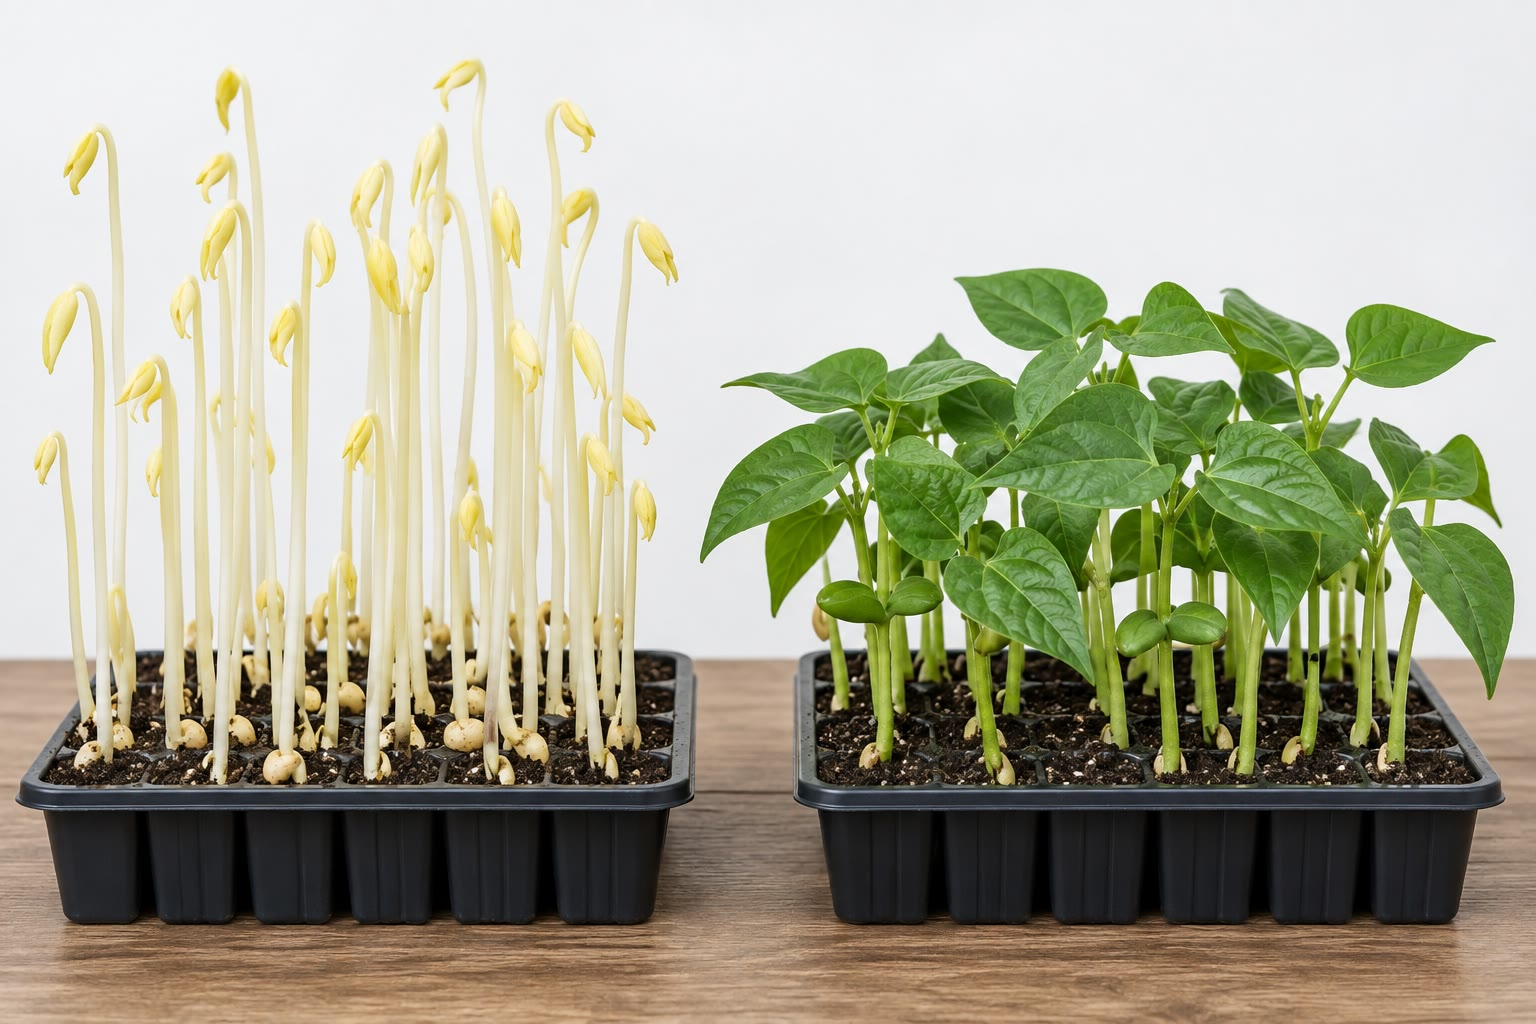
\includegraphics[width=0.56\linewidth]{images/book5/ai/b5-22-etiolated-seedlings.jpg}

{\small Des plants poussés dans l'obscurité et à la lumière~: le même
génome, deux programmes de développement, et la différence tient à un
seul photon rouge absorbé par le \omterm{def:b3:plant-molecular-physiology:photoreceptors}{phytochrome}.}
\end{omfigure}

\section{Les hormones à l'échelle moléculaire}

\begin{definition}[Les hormones végétales et leurs récepteurs]\label{def:b3:plant-molecular-physiology:hormones}
\index{auxine}\index{TIR1}\index{gibbérelline}\index{DELLA}\index{acide abscissique}\index{éthylène}\index{cytokinine}\index{brassinostéroïde}
Le volume de première année a décrit ce que font les \omterm{def:b3:endocrinology:hormone}{hormones}
végétales~; voici comment elles sont entendues. Plusieurs agissent par
\emph{destruction réglée}. L'\emph{auxine} (l'acide indole-3-acétique)
lie la protéine à boîte F \emph{TIR1}, qu'elle colle aux répresseurs
Aux/IAA, lesquels sont alors ubiquitinés et détruits par le protéasome~:
les gènes de réponse à l'auxine qu'ils réprimaient s'allument en
quelques minutes --- l'\omterm{def:b3:endocrinology:hormone}{hormone} est une colle moléculaire, et le
récepteur fait partie de la machinerie de dégradation. La
\emph{gibbérelline} fait de même avec les répresseurs \emph{DELLA} de la
croissance, par son récepteur GID1~: les blés et les riz nains de la
révolution verte portent des protéines DELLA indestructibles, et restent
donc courts quelle que soit la gibbérelline qu'ils fabriquent. Le
\emph{jasmonate} suit la même logique avec les répresseurs JAZ.
L'\emph{acide abscissique} (ABA), l'\omterm{def:b3:endocrinology:hormone}{hormone} de la sécheresse et de la
dormance, lie les récepteurs PYR/PYL, qui inhibent alors une phosphatase
(PP2C), ce qui libère une kinase (SnRK2) qui phosphoryle des canaux
ioniques et des facteurs de transcription --- une double négation qui
rend la réponse raide. L'\emph{éthylène}, un gaz, lie dans la membrane
du réticulum des récepteurs à cuivre qui, en son absence, répriment
activement la réponse~; sa liaison les éteint, et les gènes de
mûrissement, de \omterm{def:b3:cell-cycle-apoptosis:other}{sénescence} et de stress s'allument. Les
\emph{cytokinines} agissent par des récepteurs à histidine kinase, comme
les systèmes bactériens à deux composants~; les
\emph{brassinostéroïdes}, les stéroïdes de la plante, par une kinase
réceptrice de surface et non par un \omterm{def:b3:endocrinology:hormone}{récepteur nucléaire} --- les seules
\omterm{def:b3:endocrinology:hormone}{hormones stéroïdes} au monde entendues à la surface de la cellule. Les
plantes n'ont pas de glandes~: chaque \omterm{def:b3:endocrinology:hormone}{hormone} est faite là où il la
faut, ou déplacée par des transporteurs spécifiques, et sa concentration
est fixée localement par la synthèse, la conjugaison et la destruction.
\end{definition}

\begin{theorem}[Le transport polarisé chimiosmotique de l'auxine]\label{thm:b3:plant-molecular-physiology:auxin}
\index{transport polarisé de l'auxine}\index{protéines PIN}\index{piégeage de l'anion}
L'acide indole-3-acétique est un acide faible, $\mathrm{p}K_{a} = 4.75$.
Dans l'espace pariétal à pH~$5.5$ une fraction notable est la forme
neutre IAAH, qui diffuse au travers de la membrane~; dans le cytosol à
pH~$7.2$ presque tout est l'anion IAA$^{-}$, qui ne peut sortir par
diffusion. À l'équilibre de la forme neutre de part et d'autre de la
membrane, le rapport de l'\omterm{def:b3:plant-molecular-physiology:hormones}{auxine} totale du dedans à celle du dehors vaut
\[
\frac{[\text{IAA}]_{\text{in}}}{[\text{IAA}]_{\text{out}}}
= \frac{1 + 10^{\,\mathrm{pH}_{\text{in}} - \mathrm{p}K_{a}}}{1 + 10^{\,\mathrm{pH}_{\text{out}} - \mathrm{p}K_{a}}}
\approx \frac{283}{6.6} \approx 43 :
\]
la cellule piège l'\omterm{def:b3:plant-molecular-physiology:hormones}{auxine} d'un facteur quarante. Celle-ci ne peut sortir
que par les transporteurs d'efflux \emph{PIN}, et parce que chaque
cellule place ses PIN sur une seule face --- la face basale dans la tige
--- l'\omterm{def:b3:plant-molecular-physiology:hormones}{auxine} captée de tous côtés sort par le bas, entre dans la cellule
suivante, et ainsi de suite~: une colonne de cellules de même polarité
est un convoyeur qui déplace l'\omterm{def:b3:plant-molecular-physiology:hormones}{auxine} à environ \qty{1}{cm/h} de
l'apex caulinaire vers la racine, et réorienter les PIN réoriente le
courant, ce qui explique comment le côté ombré d'une tige en vient à
tenir plus d'\omterm{def:b3:plant-molecular-physiology:hormones}{auxine} et à croître plus vite.
\end{theorem}
\begin{proof}
Henderson--Hasselbalch~: $[\text{IAA}^{-}]/[\text{IAAH}] = 10^{\,\mathrm{pH}
- \mathrm{p}K_{a}}$, donc le total vaut $= [\text{IAAH}](1 + 10^{\,\mathrm{pH} -
\mathrm{p}K_{a}})$. La forme neutre s'équilibre, $[\text{IAAH}]_{\text{in}}
= [\text{IAAH}]_{\text{out}}$~; en divisant les totaux on obtient le rapport,
$(1 + 10^{2.45})/(1 + 10^{0.75}) = 283/6.6$. Avec les PIN sur une seule
face, la seule sortie de l'anion est directionnelle~; une colonne de $n$
cellules passe le flux de proche en proche, et la vitesse mesurée, d'un
ordre de grandeur au-dessus de la diffusion sur ces distances, est celle
d'un efflux porté par un transporteur à chaque limite cellulaire.
L'hypothèse de Cholodny--Went (années 1920), selon laquelle la courbure
suit une redistribution latérale de l'\omterm{def:b3:plant-molecular-physiology:hormones}{auxine}, fut confirmée par mesure
directe dans des coléoptiles d'avoine et par l'imagerie de la
relocalisation des PIN dans des racines d'\emph{Arabidopsis} couchées
sur le côté (années 2000).
\end{proof}

\begin{omfigure}
\begin{tikzpicture}[every node/.style={font=\scriptsize}, >=stealth]
  % three cells in a column
  \foreach \y in {0,-2.2,-4.4} {
    \draw[thick, omDef, fill=omDef!8] (0,\y) rectangle (3.2,\y-1.9);
    \draw[very thick, omThm] (0.6,\y-1.9) -- (2.6,\y-1.9);
    \node[right, font=\tiny] at (3.3,\y-0.4) {cytosol pH 7,2};
    \node[right, font=\tiny] at (3.3,\y-0.8) {IAA$^{-}$ piégé};
    \draw[->, thick, omDef!70!black] (-0.6,\y-0.6) -- (0.4,\y-0.6); \node[left, font=\tiny] at (-0.6,\y-0.6) {IAAH entre};
    \draw[->, thick, omDef!70!black] (3.8,\y-1.3) -- (2.8,\y-1.3);
    \draw[->, very thick, omThm] (1.6,\y-1.5) -- (1.6,\y-2.35);
  }
  \node[left, align=right, font=\tiny] at (-0.6,-1.4) {paroi pH 5,5~:\\\qty{15}{\%} IAAH,\\\qty{85}{\%} IAA$^{-}$};
  \node[omThm, right, font=\tiny] at (3.3,-2.05) {transporteurs d'efflux PIN, face basale seulement};
  \node[above] at (1.6,0.1) {apex caulinaire~: source d'auxine};
  \node[below] at (1.6,-6.8) {vers la racine, \qty{1}{cm/h}};
  \node[right, align=left] at (5.4,-3.6) {dedans : dehors $\approx 43 : 1$\\(piégeage de l'anion)\\[3pt]sortie par les seuls PIN,\\donc la colonne est un convoyeur~;\\déplacez les PIN sur une face latérale\\et le courant tourne};
\end{tikzpicture}

{\small Le modèle chimiosmotique du \omterm{thm:b3:plant-molecular-physiology:auxin}{transport polarisé de l'auxine}.
L'acide entre par n'importe quelle face sous forme de molécule neutre,
est piégé sous forme d'anion au pH du cytosol, et ne sort que par des
transporteurs que la cellule a placés sur une seule face --- de sorte
qu'une file de cellules passe l'\omterm{def:b3:plant-molecular-physiology:hormones}{auxine} dans un seul sens.}
\end{omfigure}

\begin{example}[Gravitropisme et phototropisme]\label{ex:b3:plant-molecular-physiology:tropism}
Couchez un plant sur le côté. Dans la coiffe racinaire, des plastes
denses remplis d'amidon se déposent en quelques minutes sur la nouvelle
face inférieure des cellules de la columelle~; les transporteurs PIN3 de
ces cellules se relocalisent sur la face inférieure~; l'\omterm{def:b3:plant-molecular-physiology:hormones}{auxine} s'écoule
de préférence le long du flanc inférieur de la racine où, au-dessus de
l'optimum des cellules racinaires, elle \emph{inhibe} l'élongation, et
la racine s'incurve vers le bas. Dans la tige le même écoulement latéral
vers le côté inférieur \emph{favorise} l'élongation (l'optimum des
cellules de tige est plus élevé), et la tige s'incurve vers le haut. Le
phototropisme~: la \omterm{def:b3:plant-molecular-physiology:photoreceptors}{phototropine} du côté éclairé d'une tige modifie la
disposition des PIN de sorte que l'\omterm{def:b3:plant-molecular-physiology:hormones}{auxine} s'accumule du côté ombré, qui
croît plus vite, ce qui courbe la tige vers la lumière. Les deux
mouvements sont lents --- des heures --- parce qu'ils sont de la
croissance et non du déplacement, et tous deux sont irréversibles dans
le tissu qui a poussé. Darwin (1880) montra que la pointe d'un plant de
graminée perçoit la lumière et que la région du dessous se courbe~; Went
(1928) recueillit l'influence dans un bloc de gélose posé sur une pointe
coupée et montra qu'un bloc posé de façon asymétrique sur une tige
décapitée la faisait courber~: l'influence était une substance
diffusible, qu'on nomma ensuite \omterm{def:b3:plant-molecular-physiology:hormones}{auxine}.
\end{example}

\section{L'eau, le sel, le froid et la chaleur}

\begin{definition}[Le stress abiotique]\label{def:b3:plant-molecular-physiology:abiotic}
\index{stress hydrique}\index{ajustement osmotique}\index{stress salin}\index{acclimatation au froid}\index{protéines de choc thermique}
Une plante ne peut s'échapper, alors elle s'endurcit. La
\emph{sécheresse}~: la chute du potentiel hydrique dans les racines
déclenche la synthèse d'ABA~; l'ABA ferme les stomates en quelques
minutes et, au fil des jours, allume les gènes de l'\emph{ajustement
osmotique} (proline, sucres et autres solutés compatibles s'accumulent
et abaissent le potentiel hydrique de la cellule, qui continue ainsi de
tirer l'eau), ceux des déshydrines qui protègent les protéines, et ceux
d'une surface foliaire moindre et d'une racine plus profonde. Le
\emph{sel} est une sécheresse doublée d'un poison~: le sodium entre par
les canaux potassiques et concurrence le potassium~; les plantes
tolérantes le repompent hors des racines (la voie SOS), dans les
vacuoles (les échangeurs NHX), ou l'excrètent par des glandes foliaires,
et leur extrême, l'\emph{halophyte}, vit dans l'eau de mer. Le
\emph{froid}~: le refroidissement raidit les membranes et ralentit les
enzymes~; le gel tire l'eau des cellules vers la glace extracellulaire
et les dessèche. L'\emph{acclimatation au froid} --- une semaine de
journées fraîches --- induit les facteurs de transcription CBF, qui
allument des centaines de gènes de lipides fluidifiant les membranes, de
sucres, de protéines antigel et de déshydrines, et un seigle d'hiver qui
mourrait à \qty{-5}{\celsius} en août survit à \qty{-30}{\celsius} en
janvier. La \emph{chaleur} déplie les protéines~; en quelques minutes
après une hausse, un facteur de choc thermique libère les \emph{protéines
de choc thermique}, \omterm{def:b3:structural-biology:chaperones}{chaperons} qui les replient ou s'en débarrassent, les
mêmes familles que chez tout organisme. L'\emph{inondation} prive les
racines d'oxygène~; le riz fait des canaux à air (l'aérenchyme) et
s'allonge pour tenir ses feuilles hors de l'eau, l'\omterm{def:b3:plant-molecular-physiology:hormones}{éthylène} étant le
signal qui s'accumule quand il ne peut s'échapper dans l'eau. Beaucoup
de ces programmes se recouvrent --- l'ABA, les espèces réactives de
l'oxygène et les pointes de calcium sont des seconds messagers partagés
--- et une plante acclimatée à un stress est souvent en partie protégée
contre un autre.
\end{definition}

\begin{proposition}[Le stomate comme soupape]\label{prop:b3:plant-molecular-physiology:stomata}
\index{stomate}\index{cellule de garde}\index{conductance stomatique}\index{efficience d'utilisation de l'eau}
Une paire de \emph{\omterm{prop:b3:plant-molecular-physiology:stomata}{cellules de garde}} borde chaque ostiole~; le pore
s'ouvre quand elles captent du potassium et des anions (et fabriquent du
sucre), gonflent et s'écartent en arc, et se ferme quand elles les
perdent. La lumière bleue (les \omterm{def:b3:plant-molecular-physiology:photoreceptors}{phototropines}), un CO$_{2}$ bas et
l'humidité ouvrent~; l'obscurité, un CO$_{2}$ élevé, la sécheresse et
l'ABA ferment. La route de l'ABA~: récepteur $\to$ phosphatase inhibée
$\to$ kinase active $\to$ canaux anioniques (SLAC1) ouverts $\to$ la
membrane se dépolarise $\to$ le potassium sort par des canaux sortants
$\to$ l'eau suit $\to$ le pore se ferme, en dix minutes. Le pore est là
où se fait le grand marché de la plante~: le CO$_{2}$ diffuse vers le
dedans et la vapeur d'eau vers le dehors par le même trou, et parce que
le gradient de vapeur (une feuille à \qty{100}{\%} d'humidité au dedans
contre un air à \qty{50}{\%}) est cinquante fois plus raide que le
gradient de CO$_{2}$ (\qty{400}{ppm} au dehors, \qty{250}{} au dedans),
une feuille perd plusieurs centaines de molécules d'eau pour chaque
molécule de carbone qu'elle fixe. La \emph{\omterm{prop:b3:plant-molecular-physiology:stomata}{conductance stomatique}}
$g_{s}$ fixe les deux flux~: la transpiration $E = g_{s}\,\Delta w$ et
l'assimilation $A = (g_{s}/1.6)\,\Delta c$ (le CO$_{2}$, plus lourd,
diffuse $1.6$ fois plus lentement), de sorte que l'\emph{\omterm{prop:b3:plant-molecular-physiology:stomata}{efficience
d'utilisation de l'eau}} $A/E = \Delta c/(1.6\,\Delta w)$ dépend des
gradients et non de l'ouverture du pore~; fermer le pore abaisse les
deux flux ensemble, et élever le CO$_{2}$ interne (les plantes en
C$_{4}$, qui le concentrent) ou n'ouvrir que la nuit (les plantes CAM,
dans un air frais et humide) est la façon dont les plantes du désert
améliorent le rapport.
\end{proposition}
\begin{proof}
La loi de Fick à travers le pore pour chaque gaz, avec la même
conductance géométrique mise à l'échelle par le rapport des coefficients
de diffusion $D_{\mathrm{H_2O}}/D_{\mathrm{CO_2}} = 1.6$~; diviser les
deux flux élimine $g_{s}$. Les nombres~: $\Delta w \approx \qty{15}{mmol/mol}$
d'air à \qty{25}{\celsius} et \qty{50}{\%} d'humidité, $\Delta c \approx
\qty{150}{\micro mol/mol}$~: $A/E = 150/(1.6\times\num{15000}) = 1/160$
--- $160$ molécules d'eau par CO$_{2}$ dans ces conditions douces, $500$
en air sec. La séquence de l'action de l'ABA fut établie sur des
protoplastes de \omterm{prop:b3:plant-molecular-physiology:stomata}{cellules de garde} sous patch-clamp, le courant anionique
apparaissant en moins d'une minute après l'ABA et le mutant dépourvu de
SLAC1 ne se fermant pas.
\end{proof}

\begin{omfigure}
\begin{tikzpicture}[every node/.style={font=\scriptsize}, >=stealth]
  % pore with two guard cells
  \begin{scope}[shift={(0,0)}]
    \fill[omProp!30] (0,0) ellipse (1.4 and 0.9);
    \fill[white] (0,0) ellipse (0.5 and 0.6);
    \draw[thick, omProp!80!black] (0,0) ellipse (1.4 and 0.9); \draw[thick, omProp!80!black] (0,0) ellipse (0.5 and 0.6);
    \node[below, font=\tiny] at (0,-1.0) {ouvert~: K$^{+}$, Cl$^{-}$, malate entrés, turgescent};
    \draw[->, thick, omDef] (0,0.3) -- (0,1.5) node[above, font=\tiny] {H$_2$O sort, $E = g_{s}\Delta w$};
    \draw[->, thick, omThm] (0,1.5) ++(-1.0,0) -- ++(0,-1.2); \node[left, font=\tiny, omThm] at (-1.1,1.0) {CO$_2$ entre, $A = g_{s}\Delta c/1.6$};
  \end{scope}
  \begin{scope}[shift={(4.2,0)}]
    \fill[omProp!30] (0,0) ellipse (1.2 and 0.75);
    \draw[thick, omProp!80!black] (0,0) ellipse (1.2 and 0.75); \draw[very thick, omProp!80!black] (0,-0.5) -- (0,0.5);
    \node[below, font=\tiny] at (0,-0.9) {fermé~: ions perdus, flasque};
  \end{scope}
  \draw[->, thick] (1.6,0) -- (2.8,0) node[midway, above, font=\tiny] {ABA, obscurité,};
  \node[font=\tiny] at (2.2,-0.25) {CO$_2$ élevé};
  % ABA pathway chain
  \begin{scope}[shift={(7.0,1.7)}]
    \node[draw, rounded corners, fill=omDef!20, align=center, font=\tiny] (a) at (0,0) {l'ABA lie\\PYR/PYL};
    \node[draw, rounded corners, fill=omThm!15, align=center, font=\tiny] (b) at (0,-0.9) {phosphatase PP2C\\inhibée};
    \node[draw, rounded corners, fill=omMeth!25, align=center, font=\tiny] (c) at (0,-1.8) {kinase SnRK2\\active};
    \node[draw, rounded corners, fill=omProp!25, align=center, font=\tiny] (d) at (0,-2.7) {canal anionique SLAC1\\ouvert~: dépolarisation};
    \node[draw, rounded corners, fill=omProp!25, align=center, font=\tiny] (e) at (0,-3.6) {K$^{+}$ sort, l'eau sort,\\le pore se ferme en \qty{10}{min}};
    \draw[-|, thick] (a) -- (b); \draw[-|, thick] (b) -- (c); \draw[->, thick] (c) -- (d); \draw[->, thick] (d) -- (e);
    \node[right, font=\tiny, align=left] at (1.5,-0.9) {deux inhibitions\\en série~:\\un interrupteur raide};
  \end{scope}
\end{tikzpicture}

{\small Le stomate et le signal qui le ferme. L'eau et le dioxyde de
carbone partagent le pore, de sorte que la plante troque l'un contre
l'autre à un taux fixé par les deux gradients~; l'\omterm{def:b3:endocrinology:hormone}{hormone} de la
sécheresse ferme la soupape par une chaîne de deux inhibitions, ce qui
rend la réponse tout ou rien.}
\end{omfigure}

\begin{omfigure}
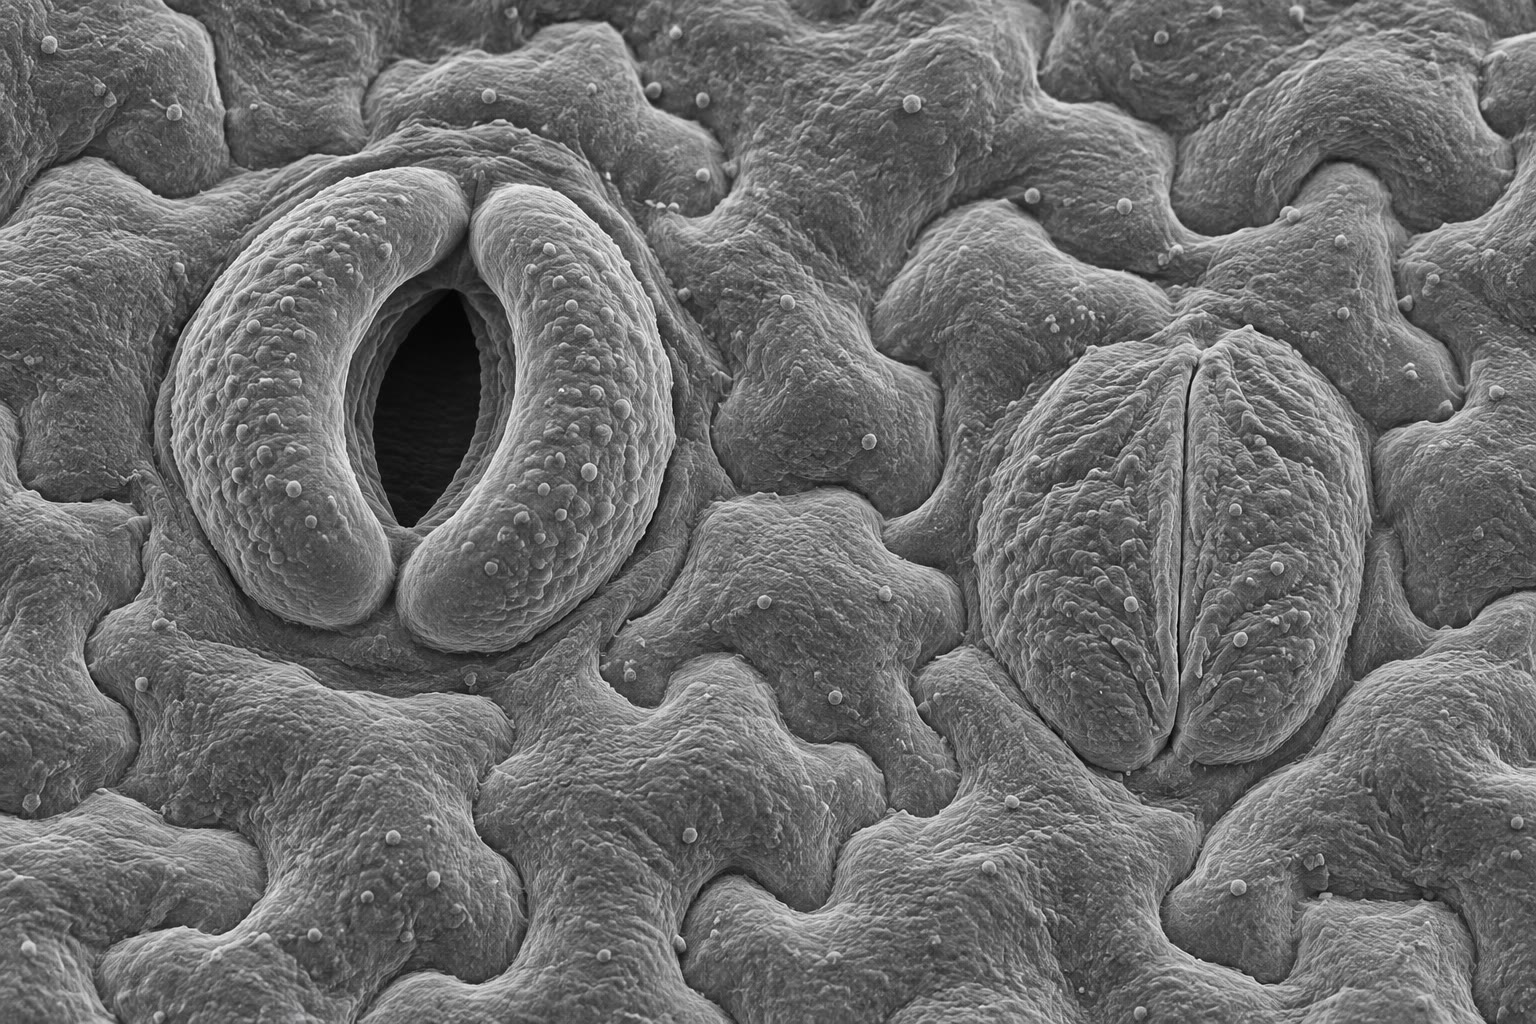
\includegraphics[width=0.46\linewidth]{images/book5/ai/b5-22-stomata-sem.jpg}\hspace{0.04\linewidth}
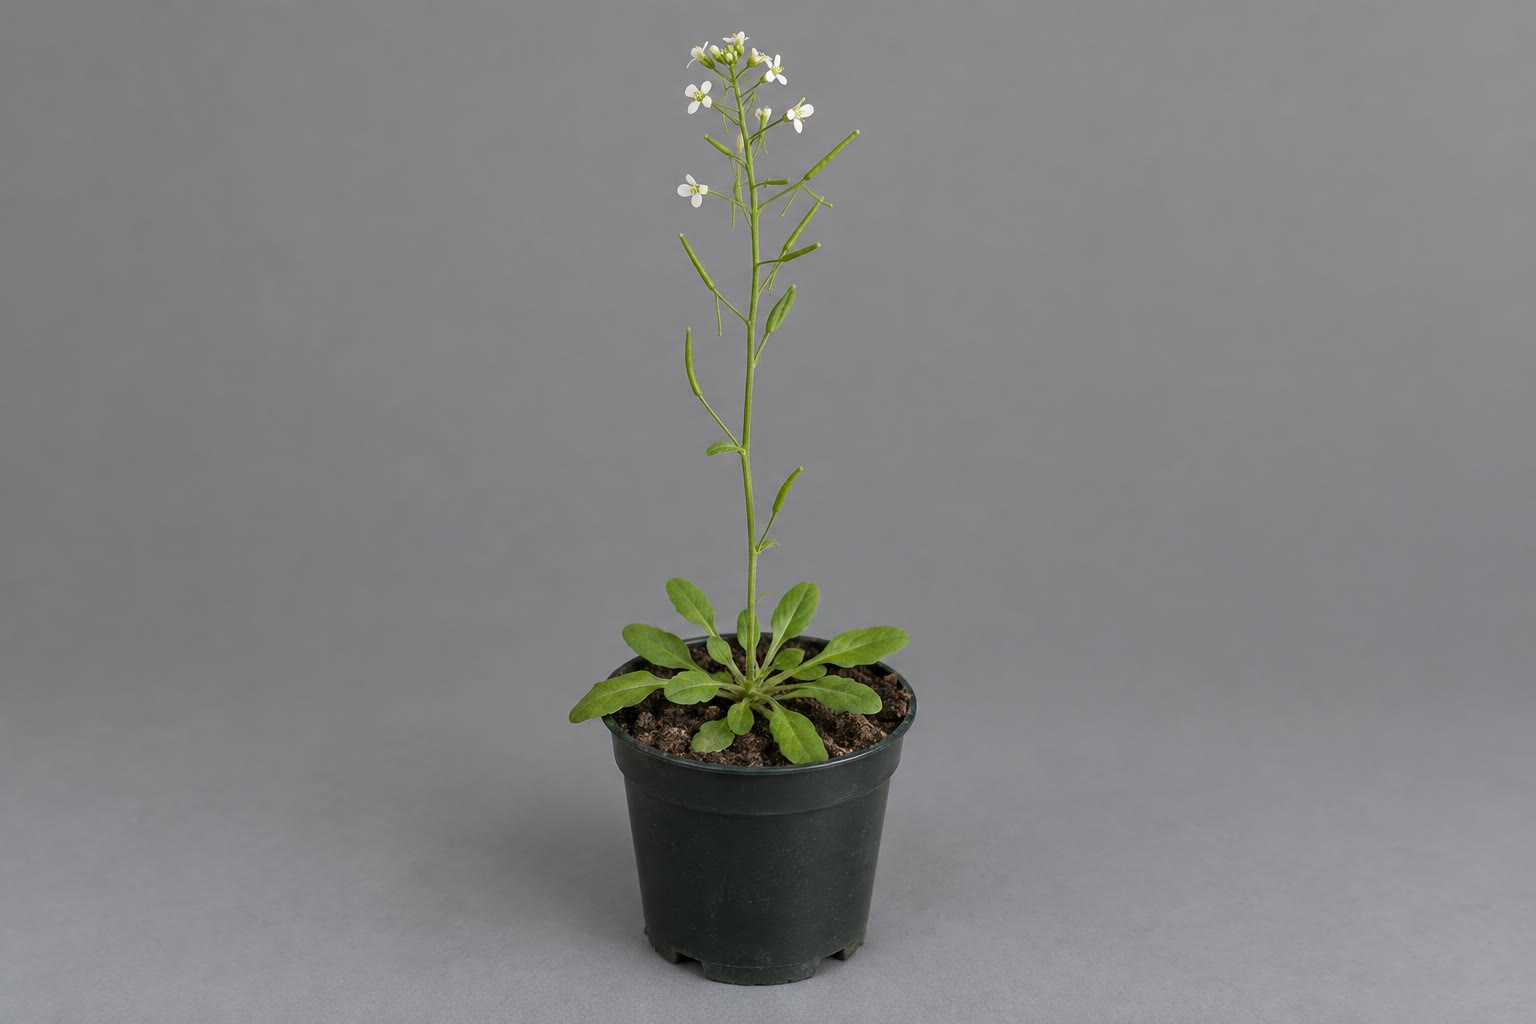
\includegraphics[width=0.46\linewidth]{images/book5/ai/b5-22-arabidopsis.jpg}

{\small À gauche~: des stomates à la surface d'une feuille, chaque pore
entre ses deux \omterm{prop:b3:plant-molecular-physiology:stomata}{cellules de garde}, certains ouverts et d'autres fermés. À
droite~: \emph{Arabidopsis thaliana}, une mauvaise herbe de bord de
route au petit génome, à la génération de six semaines et aux cent mille
lignées mutantes, chez qui la plupart des molécules de ce chapitre ont
été trouvées.}
\end{omfigure}

\section{L'immunité sans cellules immunitaires}

\begin{definition}[Les deux couches de l'immunité végétale]\label{def:b3:plant-molecular-physiology:immunity}
\index{immunité déclenchée par les motifs}\index{immunité déclenchée par les effecteurs}\index{récepteur NLR}\index{réaction hypersensible}\index{résistance systémique acquise}\index{acide salicylique}\index{acide jasmonique}
Chaque cellule végétale est sa propre cellule immunitaire. La première
couche, l'\emph{immunité déclenchée par les motifs} (PTI), emploie des
kinases réceptrices de surface qui reconnaissent des molécules communes
à des classes entières de microbes --- FLS2 lie un morceau de vingt-deux
acides aminés de la flagelline bactérienne, d'autres lient les fragments
de chitine des parois fongiques --- et lance en quelques minutes une
entrée de calcium, une bouffée d'espèces réactives de l'oxygène, des
cascades de kinases, la fermeture des stomates, l'épaississement de la
paroi par la callose, et la transcription de centaines de gènes de
défense~; elle tient la plupart des microbes en échec. Les pathogènes
qui réussissent injectent des \emph{effecteurs} --- des protéines qui
neutralisent des composants de la PTI --- et contre eux la seconde
couche, l'\emph{immunité déclenchée par les effecteurs} (ETI), aligne
des \emph{récepteurs NLR} intracellulaires (à site de liaison des
nucléotides et répétitions riches en leucine), chacun reconnaissant un
effecteur ou le dégât qu'il fait, dans l'appariement gène pour gène que
Flor a décrit chez la rouille du lin (années 1940). L'ETI est plus
rapide et plus forte que la PTI et se termine d'ordinaire par la
\emph{réaction hypersensible}~: la cellule infectée et ses voisines se
tuent, emmurant le pathogène dans du tissu mort --- les petites taches
brunes d'une feuille résistante. Les deux couches libèrent des \omterm{def:b3:endocrinology:hormone}{hormones}
qui portent l'alarme~: l'\emph{acide salicylique} contre les biotrophes
(qui se nourrissent de cellules vivantes), qui déclenche la
\emph{résistance systémique acquise} dans toute la plante pour des
semaines~; l'\emph{acide jasmonique} et l'\omterm{def:b3:plant-molecular-physiology:hormones}{éthylène} contre les
nécrotrophes (qui tuent puis se nourrissent) et les insectes broyeurs,
des jasmonates volatils avertissant les plantes voisines et attirant les
parasitoïdes des insectes. Les deux \omterm{def:b3:endocrinology:hormone}{hormones} s'antagonisent, et certains
pathogènes l'exploitent~: une bactérie qui fabrique un imitateur de
jasmonate éteint la défense salicylée qui l'aurait arrêtée.
\end{definition}

\begin{omfigure}
\begin{tikzpicture}
\begin{axis}[
  width=0.78\linewidth, height=5.4cm,
  axis x line=bottom, axis y line=left,
  xmin=0, xmax=10, ymin=0, ymax=10,
  xlabel={la course aux armements, de gauche à droite}, ylabel={amplitude de la défense},
  xlabel style={font=\small, at={(axis description cs:0.5,-0.08)}, anchor=north}, ylabel style={font=\small},
  xtick=\empty, ytick=\empty,
  clip=false,
]
\addplot[very thick, omDef] coordinates {(0,1) (1.5,5)};
\addplot[very thick, omThm] coordinates {(1.5,5) (3.2,1.8)};
\addplot[very thick, omDef] coordinates {(3.2,1.8) (4.8,8)};
\addplot[very thick, omThm] coordinates {(4.8,8) (6.4,2.2)};
\addplot[very thick, omDef] coordinates {(6.4,2.2) (8.0,8.6)};
\draw[dashed, gray] (axis cs:0,4) -- (axis cs:8.5,4); \node[font=\scriptsize, gray, anchor=west] at (axis cs:8.5,4) {seuil de résistance};
\draw[dashed, gray] (axis cs:0,7.2) -- (axis cs:8.5,7.2); \node[font=\scriptsize, gray, anchor=west] at (axis cs:8.5,7.2) {réaction hypersensible};
\node[font=\scriptsize, omDef, anchor=south west] at (axis cs:0.1,5.3) {PTI~: les récepteurs voient flagelline et chitine};
\node[font=\scriptsize, omThm, anchor=north, align=center] at (axis cs:3.2,1.6) {effecteurs injectés~:\\PTI neutralisée};
\node[font=\scriptsize, omDef, anchor=south, align=center] at (axis cs:4.8,8.2) {ETI~: un NLR reconnaît\\un effecteur};
\node[font=\scriptsize, omThm, anchor=north, align=center] at (axis cs:6.4,2.0) {effecteur perdu ou modifié~:\\reconnaissance esquivée};
\node[font=\scriptsize, omDef, anchor=south, align=center] at (axis cs:8.0,8.8) {un nouveau NLR\\apparaît};
\end{axis}
\end{tikzpicture}

{\small Le zigzag de la coévolution plante--pathogène. Les récepteurs de
surface lèvent une défense contre les molécules microbiennes communes~;
les pathogènes injectent des effecteurs qui l'étouffent~; les plantes
font apparaître des récepteurs intracellulaires des effecteurs~; les
pathogènes s'en défont ou les modifient~; et ainsi de suite, chaque
étape laissant des gènes de résistance et de virulence que sélectionneurs
et pathogènes échangent encore.}
\end{omfigure}

\begin{proof}[Faits expérimentaux]
Flor (années 1940) croisa des variétés de lin et des souches de rouille
et trouva que la résistance à chaque souche ségrégeait comme un unique
gène dominant de la plante apparié à un unique gène d'avirulence du
champignon --- la relation gène pour gène, inexpliquée cinquante ans
durant jusqu'au clonage des premiers gènes NLR (1994) et à la
démonstration que les premiers couples effecteur--récepteur se liaient
ou repéraient le dégât de l'autre. Gómez-Gómez et Boller (2000)
trouvèrent le mutant d'\emph{Arabidopsis} aveugle à la flagelline,
\emph{fls2}, et montrèrent que sa kinase réceptrice liait le peptide
flg22 à concentration nanomolaire et que le mutant était plus sensible
aux bactéries pulvérisées sur ses feuilles mais non à celles qu'on y
injectait --- le récepteur garde la surface et les stomates par où les
bactéries entrent. Ross (1961) inocula un \omterm{def:b3:virology:virus}{virus} à une feuille d'un plant
de tabac et trouva les autres feuilles résistantes une semaine plus
tard~: la \omterm{def:b3:plant-molecular-physiology:immunity}{résistance systémique acquise}, dont on montra ensuite qu'elle
demande l'\omterm{def:b3:plant-molecular-physiology:immunity}{acide salicylique}, que la plante fait par la même voie que le
parent de l'aspirine.
\end{proof}

\begin{example}[L'horloge de la plante et la durée du jour]\label{ex:b3:plant-molecular-physiology:clock}
Les plantes tiennent une \omterm{def:b3:endocrinology:clock}{horloge circadienne} de même dessin que
l'horloge animale et faite de pièces sans parenté~: des facteurs du
matin (CCA1, LHY) répriment un gène du soir (TOC1) dont le produit les
réprime, avec d'autres boucles qui rendent robuste un cycle de 24 heures
même sous lumière constante, et qui anticipent l'aube en ouvrant les
stomates et en allumant les gènes de la photosynthèse une heure avant le
soleil. La sortie la plus lourde de conséquences de l'horloge est la
mesure de la durée du jour. Chez \emph{Arabidopsis}, plante de jours
longs, l'horloge fait s'accumuler la protéine CONSTANS en fin
d'après-midi~; dans un jour long cette après-midi est encore éclairée,
le \omterm{def:b3:plant-molecular-physiology:photoreceptors}{phytochrome} et le \omterm{def:b3:plant-molecular-physiology:photoreceptors}{cryptochrome} stabilisent la protéine, et elle
allume \emph{FT} dans la feuille~; dans un jour court la protéine est
faite dans l'obscurité et détruite. La protéine FT, la florigène que les
expériences de greffe poursuivaient depuis Tchaïlakhian (1936), voyage
dans le phloème jusqu'à l'apex caulinaire et, avec un partenaire
qu'elle y trouve, convertit l'apex de faiseur de feuilles en faiseur de
fleurs. Les plantes de jours courts (riz, soja) emploient la même
horloge avec le signe inversé. Une plante lit donc le calendrier en
comparant un rythme interne à la lumière externe --- la «~coïncidence
externe~» que Bünning proposa en 1936 et que la génétique moléculaire a
rendue littérale soixante-dix ans plus tard.
\end{example}

\begin{remark}[Rester immobile, tout changer]\label{rem:b3:plant-molecular-physiology:remark}
La réponse de l'animal à un environnement mauvais est de le quitter~;
celle de la plante est de devenir une autre plante. Elle a des
récepteurs pour la couleur et la direction de la lumière, l'attraction
de la pesanteur, le potentiel hydrique de son sol, la touche du vent et
la chimie de ses ennemis~; ses \omterm{def:b3:endocrinology:hormone}{hormones} agissent en détruisant des
répresseurs, de sorte qu'un signal peut commuter un programme en
quelques minutes~; et chacune de ses cellules est son propre capteur,
son propre système immunitaire et, s'il le faut, son propre méristème
régénérateur. Les blés nains qui ont nourri un monde en croissance
étaient une protéine \omterm{def:b3:plant-molecular-physiology:hormones}{DELLA} qu'on ne pouvait dégrader~; les cultures
tolérantes à la sécheresse des décennies à venir seront, pour une bonne
part, affaire de récepteurs de l'ABA, de \omterm{prop:b3:plant-molecular-physiology:stomata}{conductance stomatique} et de
l'\omterm{prop:b3:plant-molecular-physiology:stomata}{efficience d'utilisation de l'eau} que ce chapitre a calculée.
\end{remark}

\section{Exercices}

\begin{exercise}[$\star$]\label{exo:b3:plant-molecular-physiology:1}
Énumérer les trois familles de photorécepteurs avec leurs longueurs
d'onde et une réponse pour chacune. Pourquoi une plante a-t-elle besoin
de photorécepteurs alors qu'elle a déjà la chlorophylle~?
\end{exercise}

\begin{exercise}[$\star$]\label{exo:b3:plant-molecular-physiology:2}
Expliquer comment l'\omterm{def:b3:plant-molecular-physiology:hormones}{auxine}, la \omterm{def:b3:plant-molecular-physiology:hormones}{gibbérelline} et le jasmonate partagent un
mécanisme d'action, et pourquoi cela rend la réponse rapide.
\end{exercise}

\begin{exercise}[$\star$]\label{exo:b3:plant-molecular-physiology:3}
Décrire la suite des événements depuis l'arrivée de l'ABA sur une
\omterm{prop:b3:plant-molecular-physiology:stomata}{cellule de garde} jusqu'à la fermeture du pore, et nommer le point où une
mutation laisserait la plante incapable de fermer ses stomates.
\end{exercise}

\begin{exercise}[$\star$]\label{exo:b3:plant-molecular-physiology:4}
Distinguer l'\omterm{def:b3:plant-molecular-physiology:immunity}{immunité déclenchée par les motifs} de celle déclenchée par
les effecteurs par ce qui est reconnu, où se trouve le récepteur, et
comment la réponse se termine.
\end{exercise}

\begin{exercise}[$\star\star$]\label{exo:b3:plant-molecular-physiology:5}
À l'aide de l'ajustement $\varphi \approx 0.87\,\zeta/(\zeta + 0.6)$,
calculer la fraction de Pfr en pleine lumière ($\zeta = 1.15$), sous une
feuille ($\zeta =
0.4$), sous un couvert dense ($\zeta = 0.1$) et sous une lampe à
incandescence ($\zeta = 0.7$). Pourquoi les plants poussent-ils en
hauteur sous de telles lampes~?
\end{exercise}

\begin{exercise}[$\star\star$]\label{exo:b3:plant-molecular-physiology:6}
Calculer le rapport dedans:dehors de l'\omterm{def:b3:plant-molecular-physiology:hormones}{auxine} si le pH de la paroi vaut
$5.0$ et celui du cytosol $7.5$~; puis si la paroi est acidifiée à $4.5$
(comme le font les cellules en croissance). Qu'advient-il du piégeage si
le cytosol s'acidifie à $6.5$ sous anoxie~?
\end{exercise}

\begin{exercise}[$\star\star$]\label{exo:b3:plant-molecular-physiology:7}
L'\omterm{def:b3:plant-molecular-physiology:hormones}{auxine} se déplace à \qty{1}{cm/h} à travers des cellules longues de
\qty{50}{\micro m}. Combien de cellules traverse-t-elle par heure, et
combien de temps passe-t-elle dans chacune~? Comparer au temps de
diffusion sur \qty{50}{\micro m} ($D =
\qty{5e-10}{m^2/s}$, $t \approx x^{2}/2D$) et dire quelle étape limite
le transport.
\end{exercise}

\begin{exercise}[$\star\star$]\label{exo:b3:plant-molecular-physiology:8}
Une feuille à \qty{25}{\celsius} a une fraction molaire de vapeur
interne de \qty{32}{mmol/mol} et l'air \qty{16}{mmol/mol}~; le CO$_{2}$
vaut \qty{400}{ppm} au dehors et \qty{250}{ppm} au dedans. Calculer les
molécules d'eau perdues par CO$_{2}$ fixé. Recalculer pour une plante en
C$_{4}$ dont le CO$_{2}$ interne vaut \qty{150}{ppm}, et pour un jour sec
avec un air à \qty{8}{mmol/mol}.
\end{exercise}

\begin{exercise}[$\star\star$]\label{exo:b3:plant-molecular-physiology:9}
Expliquer pourquoi une plante acclimatée au froid tolère souvent mieux
aussi la sécheresse, en nommant les signaux partagés et les molécules
protectrices partagées.
\end{exercise}

\begin{exercise}[$\star\star\star$]\label{exo:b3:plant-molecular-physiology:10}
Le \omterm{def:b3:plant-molecular-physiology:photoreceptors}{phytochrome} approche son photoéquilibre à la vitesse $k_{1} + k_{2}$
proportionnelle au flux. Si le plein soleil donne $k_{1} + k_{2} =
\qty{0.5}{s^{-1}}$, combien de temps prend le basculement sous le
\qty{1}{\%} de plein soleil de l'aube~? La Pfr revient en arrière dans
l'obscurité avec une demi-vie de \qty{2}{h}~: quelle fraction en reste-t-il
après une nuit de huit heures, et comment cela permet-il à une graine de
distinguer une brève exposition d'une journée~?
\end{exercise}

\begin{exercise}[$\star\star\star$]\label{exo:b3:plant-molecular-physiology:11}
La \omterm{def:b3:plant-molecular-physiology:immunity}{réaction hypersensible} tue peut-être une centaine de cellules par
site d'infection. Argumenter, par une estimation grossière du coût et du
bénéfice pour une feuille de $10^{7}$ cellules affrontant dix infections
par jour, pourquoi le suicide des cellules infectées est bon marché, et
pourquoi un nécrotrophe (qui se nourrit de cellules mortes) fait de cette
défense une faiblesse.
\end{exercise}

\begin{exercise}[$\star\star\star$]\label{exo:b3:plant-molecular-physiology:12}
Modéliser la coïncidence externe~: la protéine CONSTANS est faite entre
la douzième et la seizième heure après l'aube et détruite avec une
demi-vie de \qty{30}{min} dans l'obscurité mais de \qty{4}{h} à la
lumière. Estimer la protéine restante à la seizième heure dans un jour
de 16 heures et dans un jour de 10 heures (obscurité dès la dixième
heure), et expliquer comment un seuil en fait une décision de fleurir.
\end{exercise}

\section{Problème~: un plant à l'ombre}

\begin{problem}[{Problème du week-end --- un plant lu par ses molécules~:
l'équilibre du phytochrome sous un couvert, l'auxine qu'il piège et
transporte, l'eau qu'il troque contre du carbone par ses stomates, et le
coût de la défense de ses feuilles, pour finir sur la fraction de Pfr
sous le couvert, le rapport de piégeage de l'auxine et l'efficience
d'utilisation de l'eau}]
\label{pb:b3:plant-molecular-physiology:1}
Données~: ajustement du photoéquilibre $\varphi = 0.87\,\zeta/(\zeta + 0.6)$~;
pleine lumière $\zeta = 1.15$, couvert $\zeta = 0.2$~; vitesse
d'élongation de l'hypocotyle $r = r_{0}(1 - \varphi)$ avec $r_{0} = \qty{2}{mm/h}$.
\omterm{def:b3:plant-molecular-physiology:hormones}{Auxine}~: $\mathrm{p}K_{a} = 4.75$~; pH pariétal $5.5$, pH cytosolique
$7.2$~; vitesse de transport \qty{1}{cm/h}~; longueur des cellules
\qty{100}{\micro m}. Feuille~: fraction molaire de vapeur au dedans
\qty{32}{mmol/mol}, air \qty{16}{mmol/mol}~; CO$_{2}$ \qty{400}{ppm} au
dehors, \qty{250}{ppm} au dedans~; $g_{s} =
\qty{0.3}{mol\,m^{-2}\,s^{-1}}$ (vapeur d'eau)~; surface foliaire
\qty{20}{cm^2}~; \qty{12}{h} de lumière. Défense~: la \omterm{def:b3:plant-molecular-physiology:immunity}{réaction
hypersensible} tue $100$ cellules par site~; la feuille a $10^{7}$
cellules~; la PTI coûte \qty{5}{\%} de la photosynthèse quand elle est
active.

\medskip
\noindent\textbf{Partie I --- La lumière.}
\begin{enumerate}
  \item Calculer $\varphi$ en pleine lumière et sous le couvert.
  \item Les vitesses d'élongation dans chaque cas, et la longueur
        supplémentaire après \qty{48}{h} à l'ombre.
  \item La feuille d'une voisine retire \qty{90}{\%} du rouge et
        \qty{20}{\%} du rouge lointain de la lumière du jour. Calculer le
        nouveau $\zeta$ et le nouveau $\varphi$. Une seule feuille
        suffit-elle à déclencher l'\omterm{prop:b3:plant-molecular-physiology:photoequilibrium}{évitement de l'ombre}~?
  \item Expliquer pourquoi $\varphi$ est indépendant de l'intensité, et
        ce que cela signifie pour un plant à découvert un jour nuageux.
  \item Le plein soleil donne $k_{1} + k_{2} = \qty{0.5}{s^{-1}}$. Temps
        pour atteindre \qty{95}{\%} du photoéquilibre en plein soleil et
        à \qty{1}{\%} de celui-ci~?
  \item La Pfr faite dans la journée revient en arrière avec une demi-vie
        de \qty{2}{h}. Fraction restante après \qty{8}{h} et après
        \qty{14}{h} d'obscurité~; comment une plante pourrait-elle s'en
        servir comme horloge de la longueur de la nuit, et pourquoi
        est-ce une mauvaise horloge~?
\end{enumerate}

\medskip
\noindent\textbf{Partie II --- L'\omterm{def:b3:plant-molecular-physiology:hormones}{auxine}.}
\begin{enumerate}[resume]
  \item Fraction d'\omterm{def:b3:plant-molecular-physiology:hormones}{auxine} sous forme neutre IAAH dans la paroi et dans
        le cytosol.
  \item Rapport dedans:dehors à l'équilibre de l'IAAH. Si la paroi tient
        \qty{0.1}{\micro M} d'\omterm{def:b3:plant-molecular-physiology:hormones}{auxine} totale, quelle est la concentration
        cytosolique~?
  \item Cellules traversées par heure, et temps de séjour par cellule.
  \item Une tige de \qty{5}{cm} de long~: combien de temps faut-il pour
        qu'un changement d'\omterm{def:b3:plant-molecular-physiology:hormones}{auxine} à la pointe gagne la base~? Comparer à
        l'heure que met une tige à commencer de se courber vers la
        lumière, et commenter.
  \item Dans une racine gravistimulée, PIN3 se relocalise de sorte que
        le flanc inférieur reçoit \qty{60}{\%} du flux et le supérieur
        \qty{40}{\%}. Si l'élongation des cellules racinaires baisse de
        \qty{1}{\%} pour chaque \qty{1}{\%} d'\omterm{def:b3:plant-molecular-physiology:hormones}{auxine} au-dessus de la
        norme et monte d'autant en dessous, calculer les vitesses des
        deux flancs par rapport à la norme, et le sens de la courbure.
  \item Pourquoi la même asymétrie courbe-t-elle une tige dans l'autre
        sens~?
\end{enumerate}

\medskip
\noindent\textbf{Partie III --- De l'eau pour du carbone.}
\begin{enumerate}[resume]
  \item La transpiration $E = g_{s}\,\Delta w$ en \unit{mmol\,m^{-2}\,s^{-1}}.
  \item L'assimilation $A = (g_{s}/1.6)\,\Delta c$ en \unit{\micro
        mol\,m^{-2}\,s^{-1}}, et le rapport $E/A$.
  \item L'eau perdue par la feuille de \qty{20}{cm^2} dans la journée de
        12 heures, en moles et en grammes~; le carbone fixé, en moles de
        CO$_{2}$ et en grammes de glucose.
  \item L'ABA ferme les stomates à $g_{s} = \qty{0.05}{}$. Nouveaux $E$
        et $A$, et le rapport. Qu'a gagné et qu'a perdu la plante~?
  \item Une plante en C$_{4}$ tient son CO$_{2}$ interne à
        \qty{150}{ppm} avec le même $g_{s}$~: son $E/A$~? Une plante CAM
        ouvre la nuit quand $\Delta w = \qty{5}{mmol/mol}$~: son $E/A$
        avec $\Delta c =
        \qty{150}{ppm}$~?
  \item Expliquer pourquoi le rapport $E/A$ ne dépend pas de $g_{s}$, et
        ce qu'une plante peut et ne peut pas y faire.
\end{enumerate}

\medskip
\noindent\textbf{Partie IV --- La défense.}
\begin{enumerate}[resume]
  \item Dix sites d'infection par jour, chacun traité par une \omterm{def:b3:plant-molecular-physiology:immunity}{réaction
        hypersensible}~: cellules tuées par jour, en fraction de la
        feuille.
  \item Sur une vie de feuille de 60 jours, quelle fraction est
        sacrifiée~? Comparer à la perte si une infection sur dix
        s'échappait et détruisait \qty{5}{\%} de la feuille chaque fois.
  \item La PTI est active \qty{20}{\%} du temps~: coût moyen en fraction
        de la photosynthèse. Pourquoi les plantes ne la laissent-elles
        pas allumée en permanence~?
  \item Un pathogène supprime l'effecteur qu'un NLR reconnaît. Qu'y
        gagne-t-il, qu'y perd-il, et que fait ensuite la population
        végétale~?
  \item Une bactérie sécrète un imitateur du jasmonate. Quelle défense
        éteint-elle et pourquoi cela l'aide-t-il, étant donné
        l'antagonisme entre les deux voies hormonales~?
  \item Pourquoi une résistance gène pour gène dans une culture en
        monoculture est-elle souvent vaincue en quelques saisons, et que
        suggère le zigzag de faire aux sélectionneurs à la place~?
  \item Résumer~: $\varphi$ sous le couvert (question~1), le rapport de
        piégeage de l'\omterm{def:b3:plant-molecular-physiology:hormones}{auxine} (question~8) et les molécules d'eau perdues
        par CO$_{2}$ fixé (question~14).
\end{enumerate}
\end{problem}
